\documentclass[sigconf, anonymous=false, review=true, 10pt]{acmart} 

% =========== Packages ============
\usepackage{xcolor}
% \usepackage[table]{xcolor}
% \usepackage{colortbl}
% \usepackage{url}
\usepackage{xurl}
\usepackage{booktabs}
\usepackage[ruled]{algorithm2e}
\usepackage{algpseudocode}
\usepackage{enumerate}
\usepackage[english]{babel}
\usepackage{blindtext}
\usepackage[caption=false,font=footnotesize,subrefformat=parens]{subfig}
\usepackage{amsmath}
\let\Bbbk\relax
\usepackage{amssymb}
\usepackage{xspace}
\usepackage{multirow}
\usepackage{threeparttable}
\usepackage{float}
\usepackage{flafter}
\usepackage{comment}
\usepackage[skip=12pt]{caption}
\usepackage{graphicx}

% =========== Spacing Tools ============
% These removes excess margins around figures. No more manual adjustment for every figure.
% \setlength{\floatsep}{0.5mm}
% \setlength{\dblfloatsep}{0.5mm}
% \setlength{\textfloatsep}{3.0mm}
% \setlength{\dbltextfloatsep}{3.0mm}
% \setlength{\intextsep}{0.5mm}

% \abovecaptionskip 10.0pt % mm % space above caption (10.0pt)
% \belowcaptionskip 0.0pt% space below caption (0.0pt)
% \renewcommand{\baselinestretch}{0.99} % line space

% =========== Definitions & Declarations ============
\def\fig{Fig.\xspace}
\def\eqn{Eq.\xspace}
\def\sec{Sec.\xspace}
\def\tab{Tab.\xspace}

\def\ie{{\textit{i.e.}\xspace}} 
\def\eg{{\textit{e.g.}\xspace}}
\def\aka{{\textit{a.k.a.}\xspace}} 
\def\etal{{\textit{et al.}\xspace}}

\newcommand{\head}[1]{{\noindent \textbf{#1:}}}
\newcommand{\term}[1]{{\textit{#1}}}

\graphicspath{{./figures/}}
\graphicspath{{./pdf/}}
\DeclareGraphicsExtensions{.pdf,.jpeg,.png}

% =========== Editing Tools ============
\ifodd 0
\newcommand{\rev}[1]{{\color{blue}#1}} %revise of the text
\newcommand{\com}[1]{\textbf{\color{red}(COMMENT: #1)}} %comment of the text
\newcommand{\todo}[1]{\textbf{{\color{orange}(TODO: #1)}}}
\else
\newcommand{\rev}[1]{#1}
\newcommand{\com}[1]{}
\newcommand{\todo}[1]{}
\fi

% =========== Meta Info ============
\renewcommand\footnotetextcopyrightpermission[1]{} % removes footnote with conference info
\setcopyright{none}
%\setcopyright{acmcopyright}
%\setcopyright{acmlicensed}
%\setcopyright{rightsretained}
%\setcopyright{usgov}
%\setcopyright{usgovmixed}
%\setcopyright{cagov}
%\setcopyright{cagovmixed}

\settopmatter{printacmref=false, printccs=false, printfolios=false}

% DOI
\acmDOI{}

% ISBN
\acmISBN{}

%Conference
% \acmConference[Submitted for review to ACM MobiCom]{}
% \acmYear{2023}
% \copyrightyear{}
% \acmSubmissionID{\#xxx, 12+X pages}

%% {} with no args suppresses printing of the price
\acmPrice{}

\def\sysname{\textsc{GPR}\xspace}
% =========== Body ============
\begin{document}

\title[\sysname]{Group Project: Wi-Fi Sensing via ESP32-C5}


%%%%%%%%%%%%%%%%%%%%%%%%%%%%%%%%%%%%%%%%%%%%%%%%%%%%%%%%%%%
%%%%%%%%%%%%%%%%%%%% YOUR NAME %%%%%%%%%%%%%%%%%%%%%%%%%%%
\author{Name}
\email{Email}
\affiliation{%
    \institution{Your GROUP NAME}
    \city{Hong Kong}
    \country{}
}

\author{Name}
\email{Email}
\affiliation{%
    \institution{Your GROUP NAME}
    \city{Hong Kong}
    \country{}
}

\author{Name}
\email{Email}
\affiliation{%
    \institution{Your GROUP NAME}
    \city{Hong Kong}
    \country{}
}

\author{Name}
\email{Email}
\affiliation{%
    \institution{Your GROUP NAME}
    \city{Hong Kong}
    \country{}
}
%%%%%%%%%%%%%%%%%%%%%%%%%%%%%%%%%%%%%%%%%%%%%%%%%%%%%%%%%%%



% The default list of authors is too long for headers}
\renewcommand{\shortauthors}{\sysname}

% \begin{abstract}

% \end{abstract}

\maketitle
\section{Individual Contribution}
You should list the contribution and statements in the table \ref{individual contribution}.

\begin{table}[!h]
\centering
\caption{Individual Contribution}
\label{individual contribution}
    \begin{tabular}{ccc}
    \toprule
    \textbf{Name} & \textbf{UID} & \textbf{Contribution Statement} \\
    \midrule
    A & a & a\%, a's role and contributions here. \\
    B & b & b\%, b's role and contributions here. \\
    C & c & c\%, c's role and contributions here. \\
    D & d & d\%, d's role and contributions here. \\
    \bottomrule
    \end{tabular}
\end{table}

\section{Overall Result}
\subsection{Evaluation Result}
You should enter your results of the \textbf{evaluation dataset} of both tasks in the table \ref{eval}, e.g., accuracy for motion detection, and median MAE for breathing rate estimation.

\begin{table}[!h]
\centering
\caption{Overall Evaluation Result.}
\label{eval}
    \begin{tabular}{cc}
    \toprule
    \textbf{Evaluation Dataset} & \textbf{Result} \\
    \midrule
    Motion Detection & Your Accuracy (\%) \\
    Breathing Rate Estimation & Your median MAE (BPM) \\
    \bottomrule
    \end{tabular}
\end{table}

\subsection{Test Result}
\subsubsection{Breathing Rate Test}
You should plot three figures, e.g., Fig.\ref{res1}-\ref{res3}, of your estimated breathing rate, whose titles are the three test files, and put them here. 
\begin{figure}[!h]
    \centering
    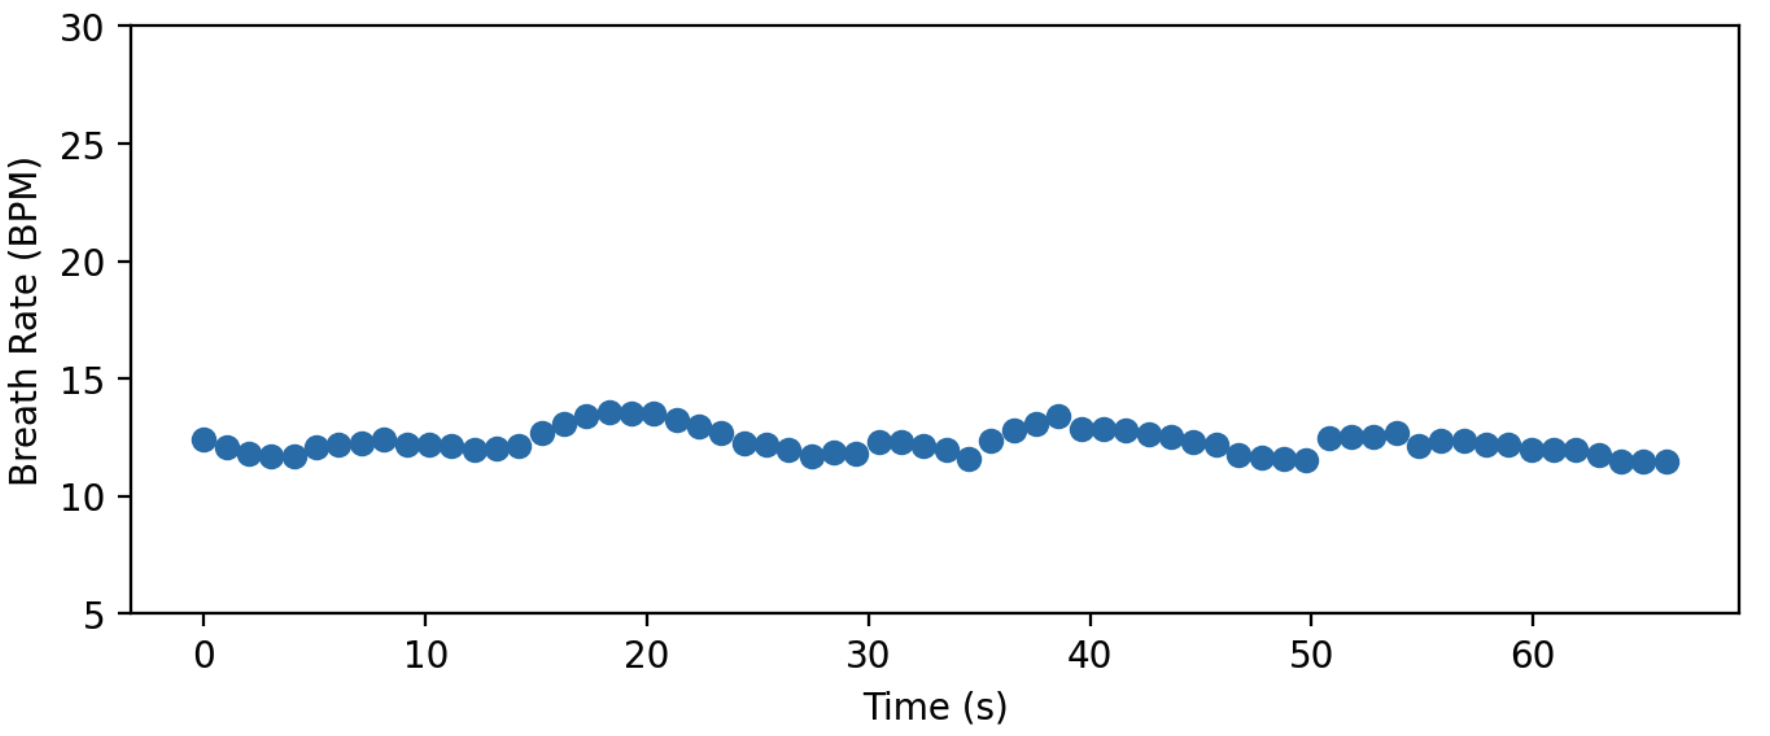
\includegraphics[width=0.5\linewidth]{fig/Exp.jpg}
    \caption{Estimated Respiration for \rm{193342.csv}.}
    \label{res1}
\end{figure}

\begin{figure}[!h]
    \centering
    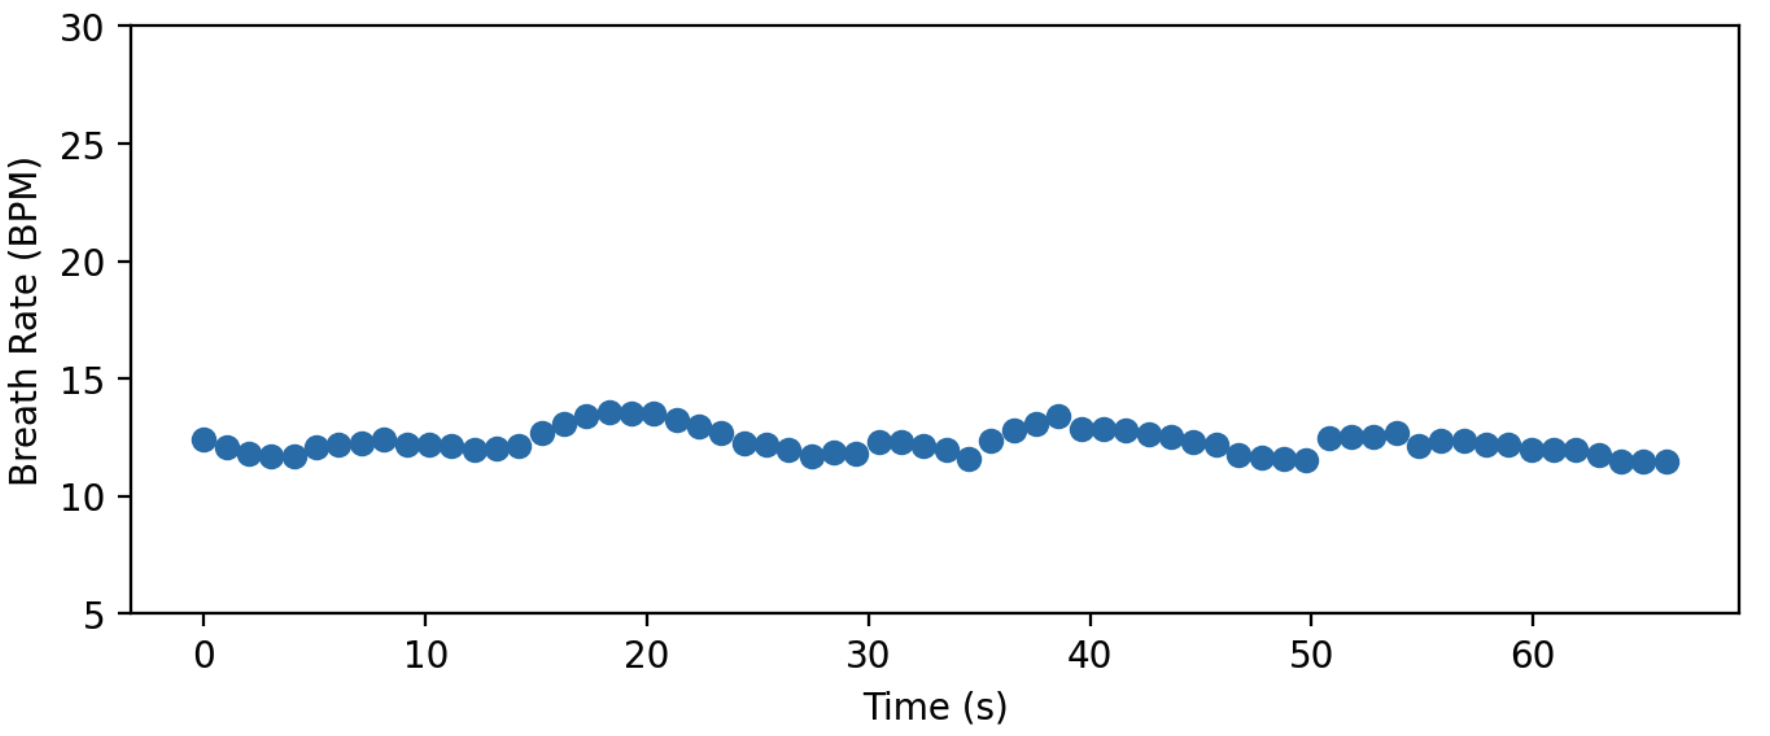
\includegraphics[width=0.5\linewidth]{fig/Exp.jpg}
    \caption{Estimated Respiration for \rm{200223.csv}.}
    \label{res2}
\end{figure}

\begin{figure}[!h]
    \centering
    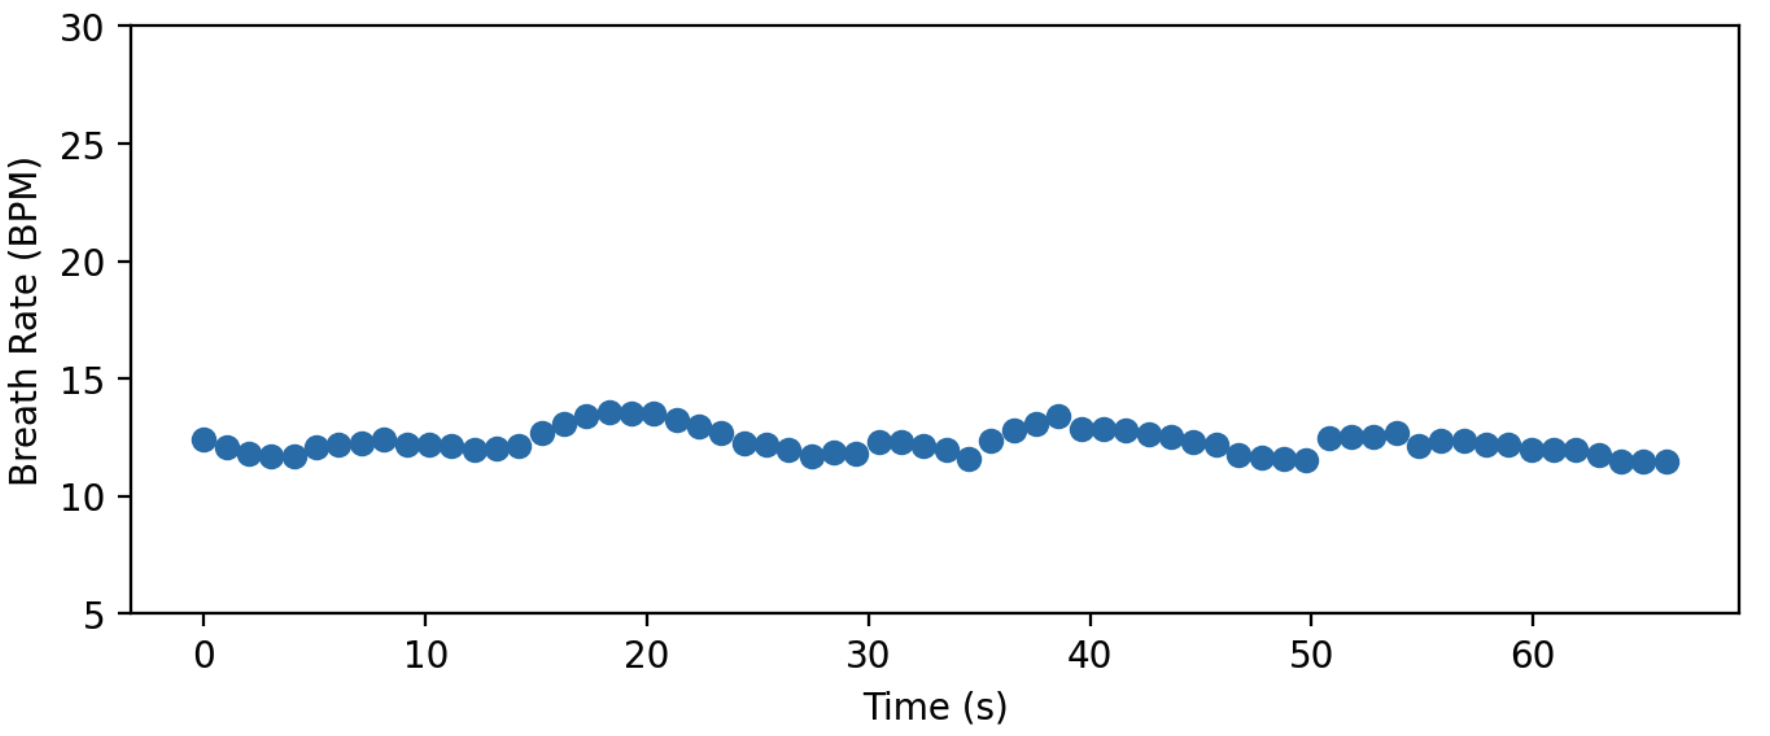
\includegraphics[width=0.5\linewidth]{fig/Exp.jpg}
    \caption{Estimated Respiration for \rm{201424.csv}.}
    \label{res3}
\end{figure}

\subsubsection{Motion Test}
Enter your result (1 for motion detected, 0 for no) in the table \ref{test motion}.

\begin{table}[!h]
\centering
\caption{Test Result of Motion Detection.}
\label{test motion}
    \begin{tabular}{cc|cc}
    \toprule
    \textbf{File Name} & \textbf{Result} & \textbf{File Name} & \textbf{Result} \\
    \midrule
    205713.csv &  & 205723.csv & \\
    205733.csv &  & 205803.csv & \\
    205822.csv &  & 205834.csv & \\
    205845.csv &  & 205855.csv & \\
    205906.csv &  & 205928.csv & \\
    205943.csv &  & 205958.csv & \\
    210036.csv &  & 210911.csv & \\
    210928.csv &  & 210942.csv & \\
    211010.csv &  & 211023.csv & \\
    211035.csv &  & 211055.csv & \\
    211107.csv & \\
    \bottomrule
    \end{tabular}
\end{table}


\clearpage
\newpage
\section{System Design}
\section{Results Visualization}
\section{Analysis}

% add whatever you want


\bibliographystyle{ACM-Reference-Format}
\bibliography{refs}

% \input{appendix}

\end{document}


% Notes: 
% 1. Put final pdf figures under ./odf folder, and other editable/original figures in any format under ./fig folder. 
% 2. Use labels with prefix:
%    - sec: for sections (including subsections), e.g., \label{sec:intro}
%    - fig: for figures (including subfigures), e.g., \label{fig:architecture}
%    - tab: for tables, e.g, \label{tab:summary}
%    - eqn: for equations, e.g, \label{eqn:csi}
% 3. Reference equations with \eqref
% 4. Don't separate sections into different files (except for appendices, if any)
% 5. When changing a template (e.g., to submit to a different venue), create a different main.tex file like this one, and keep the entire project the same.